% * * * * * * * * * * * * * * * * * * * * * * * * * * * * * * * * * * * * * * *
% * * * * * * * * * * * * * * * * * ENTETE  * * * * * * * * * * * * * * * * * *
% * * * * * * * * * * * * * * * * * * * * * * * * * * * * * * * * * * * * * * *

\documentclass[9pt]{beamer}

\include{settings}

% * * * * * * * * * * * * * * * * * * * * * * * * * * * * * * * * * * * * * * *
% * * * * * * * * * * * * * *  DEBUT DOCUMENT * * * * * * * * * * * * * * * * *
% * * * * * * * * * * * * * * * * * * * * * * * * * * * * * * * * * * * * * * *

\begin{document}
	\definecolor{MyGreen}{rgb}{0.0,0.5,0.0}
	%\input{part_1}
	%\input{part_2}



\begin{frame}
	\center Work achievement 
	\center Document Analysis Group\vspace{2em}
	\titlepage
	\thispagestyle{empty}
	\begin{center}
		%\includegraphics[height=30mm]{unejolieimage.jpg}
	\end{center}
%	\textit{\small christophe.rigaud@etud.univ-angers.fr}
%	\begin{flushleft}
%		Supervisor: Jean-Baptiste FASQUEL
%	\end{flushleft}	
		\includegraphics[trim= 0mm 0mm 0mm 0mm, clip, width=3em]{image/LogoL3i.png}\hspace{18em}
		\includegraphics[width=3cm]{image/logo_cvc_centrevisio.png}\vspace{1em}

		\tiny	Supervisors: Dimosthenis Karatzas, Joost van de Weijer \hspace{19em}Jean-Christophe Burie, Jean-Marc Ogier 

\end{frame}

% * * * * * * * * * * * * * * * * * * * * * * * * * * * * * * * * * * * * * * * Slide

\begin{frame} 
	\begin{center}{\Large Plan }\end{center}

	\thispagestyle{empty}
	\begin{columns}[c]
		\column{15em}
		\tableofcontents[hideallsubsections]
		\column{15em}
			%\framebox{\includegraphics[trim= 0mm 0mm 0mm 0mm, clip, width=1.0\textwidth]{image/sl_0_2.png}}
	\end{columns}

	\setcounter{page}{0}
\end{frame}

%%%%%%%%%%%%%%%%%%%%%%%%%%%%%%%%%%%%%%%%%%%%%%%%%%%%%%%%%%%%%%%%%%%%%%%%%%%%%%% Section

\section{Introduction}

	\subsection[Context]{Context}
		\begin{frame}
			\frametitle{Context}			
			\begin{columns}[c]
			\column{15em}
				\framebox{\includegraphics[trim= 0 0 0 0, clip, height=1.4\textwidth]{image/ROUDIER_LESTERRESCREUSEES_010.jpg}}
% 				\begin{chronology}[5]{1983}{2010}{3ex}{\textwidth}
% 				\event{1984}{one}
% 				\event[1985]{1986}{two}
% 				\event{\decimaldate{25}{12}{2001}}{three}
% 				\end{chronology}

				\column{15em}
\framebox{\includegraphics[trim= 0 0 0 0, clip, height=1.4\textwidth]{image/MCCAY_LITTLENEMO_001.jpg}}
% 				\framebox{\includegraphics[trim= 0mm 0mm 0mm 0mm, clip, width=1.0\textwidth]{image/lisa_office.JPG}}\vspace{1em}
% 				\framebox{\includegraphics[trim= 0mm 0mm 0mm 0mm, clip, width=1.0\textwidth]{image/image_ct.jpg}}\vspace{1em}		
% 				\framebox{\includegraphics[trim= 0mm 0mm 0mm 0mm, clip, width=1.0\textwidth]{image/body.png}}
			\end{columns}
			\footnotetext[1]{ McCay, Little nemo, \emph{Slumberland}, 1905}
			\footnotetext[2]{ Nicolas Roudier, \emph{Les terres creusées}, 2011}
			\end{frame}

% * * * * * * * * * * * * * * * * * * * * * * * * * * * * * * * * * * * * * * * Slide

	\subsection[Threshold]{Optimal threshold selection}
		\begin{frame}
		\frametitle{Optimal threshold selection}
		%Initial image: 
		\begin{columns}[c]
		\column{10em}
			\framebox{\includegraphics[trim= 600px 20px 500px 400px, clip, width=1\textwidth]{image/bin_50.png}}\vspace{1em}
			%\framebox{\includegraphics[trim= 600px 20px 500px 400px, clip, width=0.5\textwidth]{image/mask_bone}}
			\column{0.1em}
			$\Rightarrow$
			\column{10em}
			\framebox{\includegraphics[trim= 600px 20px 500px 400px, clip, width=1.0\textwidth]{image/bin_100.png}}\vspace{1em}
			%\framebox{\includegraphics[trim= 10mm 10mm 10mm 30mm, clip, width=0.5\textwidth]{image/int_0_0_2}}			
			\column{0.1em}
			$\Rightarrow$
			\column{10em}
			\framebox{\includegraphics[trim= 600px 20px 500px 400px, clip, width=1.0\textwidth]{image/bin_200.png}}\vspace{1em}
		\end{columns}
		
		\end{frame}
		
% * * * * * * * * * * * * * * * * * * * * * * * * * * * * * * * * * * * * * * * Slide

	\subsection[Letter1]{Letter extraction 1}
		\begin{frame}
		\frametitle{Letter extraction}

			\begin{block}{Black on white connected components (CC) selection rules}
				\begin{enumerate}
					\item high contrast ratio
					\item no overlapping
					\item surrounded by other CC similar in height
				\end{enumerate}

			\end{block}
		\begin{columns}[c]
			\column{15em}%trim=l b r t  width=0.5\textwidth, 
			  \framebox{\includegraphics[trim= 0 120px 20px 25px, clip, height=0.7\textwidth]{image/bright.png}}\vspace{1em}
			  %\framebox{\includegraphics[trim= 600px 20px 500px 400px, clip, width=0.5\textwidth]{image/mask_bone}}
			\column{15em}
			  \framebox{\includegraphics[trim= 0 120px 20px 25px, clip, height=0.7\textwidth]{image/overlap.png}}\vspace{1em}
		\end{columns}
		
		\end{frame}


% * * * * * * * * * * * * * * * * * * * * * * * * * * * * * * * * * * * * * * * Slide

	\subsection[Letter2]{Letter extraction 2}
		\begin{frame}
		\frametitle{Letter extraction}

			\begin{block}{Black on white connected components (CC) selection rules}
				\begin{enumerate}
					\item high contrast ratio
					\item no overlapping
					\item surrounded by other CC similar in height
				\end{enumerate}

			\end{block}
		\begin{columns}[c]
			\column{15em}%trim=l b r t  width=0.5\textwidth, 
			  \framebox{\includegraphics[trim= 0 120px 20px 25px, clip, height=0.7\textwidth]{image/surroundd.png}}\vspace{1em}
			  %\framebox{\includegraphics[trim= 600px 20px 500px 400px, clip, width=0.5\textwidth]{image/mask_bone}}
			\column{15em} 
			  \framebox{\includegraphics[trim= 0 0px 0px px, clip, height=0.7\textwidth]{image/4_direction.png}}\vspace{1em}
		\end{columns}
		
>		\end{frame}

% * * * * * * * * * * * * * * * * * * * * * * * * * * * * * * * * * * * * * * * Slide

	\subsection[Line]{Letter to lines}
		\begin{frame}
		\frametitle{Letter to lines}
		\begin{center}	
		  \framebox{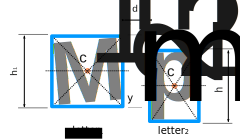
\includegraphics[trim= 200px 280px 300px 200px, clip, width=0.80\textwidth]{image/letter_position.pdf}}\vspace{1em}
		\end{center}
		
		\begin{block}{Horizontal and vertical alignment}

			\begin{enumerate}
				\item $d<Max(h1,h2)$
				\item $c2_y \in [y1_{min},y1_{max}]$
			\end{enumerate}
			
		\end{block}
		
		
		\end{frame}

% * * * * * * * * * * * * * * * * * * * * * * * * * * * * * * * * * * * * * * * Slide


%%%%%%%%%%%%%%%%%%%%%%%%%%%%%%%%%%%%%%%%%%%%%%%%%%%%%%%%%%%%%%%%%%%%%%%%%%%%%%% Section

\section{Experiments and results}
	\subsection[Dataset]{Dataset}
	\begin{frame}
		\frametitle{Dataset}
		\begin{center}	
		  \framebox{\includegraphics[trim= 0 0 0 0, clip, width=0.90\textwidth]{image/dataset.jpg}}\vspace{1em}
		\end{center}
		\begin{block}{}
			%Graphical representation of topologic and photometric relations between all the regions of an image :
			\begin{enumerate}
				\item Available at http://dagdata/documents/ ``Comics''
				\item 100 pages from 20 different authors
				\item > 5000 text lines
			\end{enumerate}					
		\end{block}
		

	\end{frame}
	
% * * * * * * * * * * * * * * * * * * * * * * * * * * * * * * * * * * * * * * * Slide

	\subsection[Ground truth]{Ground truth}
	\begin{frame}
		\frametitle{Ground truth}
		\begin{center}	
		  \framebox{\includegraphics[trim= 0 0 0 0, clip, width=0.90\textwidth]{image/gt_tool.png}}\vspace{1em}
		\end{center}
		\begin{block}{}
			%Graphical representation of topologic and photometric relations between all the regions of an image :
			\begin{enumerate}
				\item Tool from L3i laboratory (La Rochelle, France)
				\item 20/100 pages
				\item Line level
			\end{enumerate}				
		\end{block}
		

	\end{frame}

% * * * * * * * * * * * * * * * * * * * * * * * * * * * * * * * * * * * * * * * Slide

\subsection[Results]{Results}
	\begin{frame}
		\frametitle{Results}
		\begin{center}	
		  \framebox{\includegraphics[trim= 0 0 0 0, clip, width=0.90\textwidth]{image/evaluation.png}}\vspace{1em}
		\end{center}
		\begin{block}{}
					\begin{enumerate}
						\item ICDAR 2011 Robust Reading Competition - Challenge 1: Reading Text in Born-Digital Images (Web and Email)\footnotemark[1]
					\end{enumerate}					
				\end{block}
		
%		\vspace{2em}
%		\alert{Each segmented structure provides a mask that we apply on the original image.}
		\footnotetext[1]{ D. Karatzas, S. Robles Mestre, J. Mas, F. Nourbakhsh, P. Pratim Roy, \emph{In Proc. 11th International Conference of Document Analysis and Recognition}, 2011}

	\end{frame}	
	
%%%%%%%%%%%%%%%%%%%%%%%%%%%%%%%%%%%%%%%%%%%%%%%%%%%%%%%%%%%%%%%%%%%%%%%%%%%%%%% Section

\section[Conclusion]{Conclusion}
	\subsection[Conclusion]{Conclusion}
	\begin{frame}
			\frametitle{Conclusion & perspectives}

		\begin{columns}[c]
			\column{15em}%trim=l b r t  width=0.5\textwidth, 
			  \begin{block}{Before (1/05/12)}
				  \begin{enumerate}
					  \item Frame + text extraction\footnotemark[1]
					  \item 5 ground truth pages
				  \end{enumerate}
				\end{block}
			\column{15em} 
			  \begin{exampleblock}{After (27/07/12)}
				  \begin{enumerate}
					  \item Improved text extraction
					  \item 20 ground truth pages
					  \item Text validation
					  \item 1 publication (in progress)
					  \item Balloon detection
				  \end{enumerate}
				\end{exampleblock}
		\end{columns}

		  \begin{alertblock}<2>{Thanks!}
				  \begin{enumerate}
					  \item Centre de Visión per Computador
					  \item Document Analysis Group
				  \end{enumerate}
				\end{alertblock}
				
				
	\footnotetext[1]{ Rigaud, C., Tsopze, N., Burie, J.-C., and Ogier, J.-M., Robust frame and text extraction from comic books \emph{Lecture Note for Computer Science
GREC'11}, 2011}
	\end{frame}
% 	\subsection[Balloon]{Balloon detection}
% 		\begin{frame}[hide]
% 			\frametitle{Balloon detection}
% 		\begin{center}	
% 		  \framebox{\includegraphics[trim= 0 0 0 0, clip, width=0.90\textwidth]{image/balloon_real.png}}\vspace{1em}
% 		\end{center}
% 
% 		\footnotetext[1]{ Lubbin, Les bulles du labo, \emph{Episode 5}, 2012}
% 		\end{frame}
		
% * * * * * * * * * * * * * * * * * * * * * * * * * * * * * * * * * * * * * * * Slide




	%\bibliographystyle{plain}							% ordre alphabétique et les numérote en conséquence.
	%\bibliographystyle{unsrt}							% trie les entrées par ordre d’apparition dans le texte.

	%\bibliographystyle{natbib}
	%\bibliography{bibliography}
	%\bibliographystyle{alpha}
	%\bibliography{bibi.bib}
%	\begin{thebibliography}{10}
%		\bibitem{Goldbach1742}[Goldbach, 1742]
%		  Christian Goldbach.
%		  \newblock A problem we should try to solve before the ISPN '43 deadline,
%		  \newblock \emph{Letter to Leonhard Euler}, 1742.
%	\end{thebibliography}

\end{document}

% * * * * * * * * * * * * * * * * * * * * * * * * * * * * * * * * * * * * * * *
% * * * * * * * * * * * * * * * * FIN * * * * * * * * * * * * * * * * * * * * *
% * * * * * * * * * * * * * * * * * * * * * * * * * * * * * * * * * * * * * * *

